%% 
%% Copyright 2007, 2008, 2009 Elsevier Ltd
%% 
%% This file is part of the 'Elsarticle Bundle'.
%% ---------------------------------------------
%% 
%% It may be distributed under the conditions of the LaTeX Project Public
%% License, either version 1.2 of this license or (at your option) any
%% later version.  The latest version of this license is in
%%    http://www.latex-project.org/lppl.txt
%% and version 1.2 or later is part of all distributions of LaTeX
%% version 1999/12/01 or later.
%% 
%% The list of all files belonging to the 'Elsarticle Bundle' is
%% given in the file `manifest.txt'.
%% 

%% Template article for Elsevier's document class `elsarticle'
%% with numbered style bibliographic references
%% SP 2008/03/01

\documentclass[preprint,12pt,a4paper]{elsarticle}

%% Use the option review to obtain double line spacing
%% \documentclass[authoryear,preprint,review,12pt]{elsarticle}

%% For including figures, graphicx.sty has been loaded in
%% elsarticle.cls. If you prefer to use the old commands
%% please give \usepackage{epsfig}

%% The amssymb package provides various useful mathematical symbols
\usepackage{amssymb}
\usepackage{hyperref}
\usepackage{xcolor}
\setlength{\parindent}{0pt}
%% The amsthm package provides extended theorem environments
%% \usepackage{amsthm}
\usepackage{mdframed}

\newmdenv[
  linewidth=1pt,
  linecolor=black,
  topline=true,
  bottomline=true,
  rightline=true,
  leftline=true,
  innertopmargin=8pt,
  innerbottommargin=8pt,
  innerleftmargin=10pt,
  innerrightmargin=10pt,
  skipabove=10pt,
  skipbelow=10pt
]{highlightbox}
%% The lineno packages adds line numbers. Start line numbering with
%% \begin{linenumbers}, end it with \end{linenumbers}. Or switch it on
%% for the whole article with \linenumbers.
%\usepackage{lineno}

\journal{SoftwareX}

\begin{document}
\renewcommand{\labelenumii}{\arabic{enumi}.\arabic{enumii}}

\begin{frontmatter}
 
%% Title, authors and addresses

%% use the tnoteref command within \title for footnotes;
%% use the tnotetext command for theassociated footnote;
%% use the fnref command within \author or \address for footnotes;
%% use the fntext command for theassociated footnote;
%% use the corref command within \author for corresponding author footnotes;
%% use the cortext command for theassociated footnote;
%% use the ead command for the email address,
%% and the form \ead[url] for the home page:
%% \title{Title\tnoteref{label1}}
%% \tnotetext[label1]{}
%% \author{Name\corref{cor1}\fnref{label2}}
%% \ead{email address}
%% \ead[url]{home page}
%% \fntext[label2]{}
%% \cortext[cor1]{}
%% \address{Address\fnref{label3}}
%% \fntext[label3]{}

\title{TALL: Text Analysis for All -- an interactive \textsf{R}-Shiny application for exploring, modeling, and visualizing textual data}

%% use optional labels to link authors explicitly to addresses:
%% \author[label1,label2]{}
%% \address[label1]{}
%% \address[label2]{}

\author[label1,label4]{Massimo Aria\corref{cor}}
\ead{aria@unina.it}
\author[label1,label4]{Maria Spano}
\author[label1,label4]{Luca D'Aniello}
\author[label2,label4]{Corrado Cuccurullo}
\author[label3,label4]{Michelangelo Misuraca}
\cortext[cor]{Corresponding author}
\address[label1]{Dep. of Economics \& Statistics, University of Naples Federico II, Naples, Italy}
\address[label2]{Dep. of Economics, University of Campania Luigi Vanvitelli, Capua (CE), Italy}
\address[label3]{Dep. of Management \& Innovation Systems, University of Salerno, Fisciano (SA), Italy}
\address[label4]{K-Synth, Naples, Italy}

\begin{abstract}
Analyzing unstructured textual data is essential across disciplines, but often requires programming skills that many researchers lack. TALL (\textit{Text Analysis for All}) is an interactive \textsf{R}-Shiny application that unifies data import, cleaning, pre-processing, statistical analysis, and visualization into a single tool. It supports tokenization, lemmatization and Part-of-Speech (PoS) tagging for analyses in multiple languages. It includes topic modeling, correspondence and cluster analysis, co-occurrence networks, polarity detection, word embedding and text summarization. Designed for accessibility and reproducibility, TALL enables non-programmers to perform advanced text analysis efficiently and effectively. This article outlines the architecture and functionalities, demonstrating its use through illustrative examples.
\end{abstract}

\begin{keyword}
\textsf{R}-Shiny app\sep NLP\sep Text mining\sep Data visualization, \sep TALL

\end{keyword}

\end{frontmatter}

%\linenumbers

\section*{Metadata}

\begin{table}[!ht]
\begin{tabular}{|p{6.5cm}|p{6.5cm}|}
\hline
%\textbf{Code metadata description} & \textbf{Metadata} \\
%\hline
Current code version & \textit{v0.5.0} \\
\hline
Permanent link to code/repository used for this code version & \url{https://github.com/massimoaria/tall} \\
\hline
Permanent link to Reproducible Capsule & \textit{Not Applicable}\\
\hline
Legal Code License & \textit{MIT License} \\
\hline
Code versioning system used & \textit{Git} \\
\hline
Software code languages, tools, and services used & \textit{R}, \textit{R Shiny}, \textit{Google Gemini} \\
\hline
Compilation requirements, operating environments \& dependencies & 
\textit{R} ($\mathit{\geq 3.5.0}$), \textit{shiny}; \textit{Dependencies}: \textit{ca, igraph, pdftools, plotly, textrank, topicmodels, udpipe, umap, visNetwork, word2vec} \\
\hline
If available, link to developer documentation/manual & \url{https://www.tall-app.com} \\
\hline
Support email for questions & \href{mailto:aria@unina.it}{aria@unina.it} \\
\hline
\end{tabular}
%\caption{Code metadata}
\label{codeMetadata} 
\end{table}

\section{Motivation and significance}
The exponential growth of digital text has transformed how knowledge is generated, disseminated, and interpreted across scientific and professional domains \cite{ign16}. From scholarly publications and policy documents to online reviews and social media posts, textual data represent a vast empirical resource for understanding complex social, cultural, and technological phenomena. Extracting structured and reproducible insights from these sources, however, requires sophisticated \textit{Natural Language Processing} (NLP) and text mining techniques that demand programming expertise, advanced computational environments, and the ability to manage heterogeneous datasets. Consequently, many researchers—particularly in the social sciences, humanities, and applied disciplines—face technical barriers that limit systematic and replicable text analysis. This methodological divide constrains discovery and exacerbates reproducibility challenges in data-intensive research.

The TALL (\textit{Text Analysis for All}) application was designed to bridge this gap by providing a transparent, interactive, and code-free platform for textual analysis. Developed entirely in \textsf{R} with the Shiny environment, TALL integrates data import, pre-processing, analysis, and visualization into a single workflow. It supports tokenization, PoS tagging, and lemmatization in multiple languages, and includes quantitative techniques such as co-word analysis \cite{for16,ari22}, topic modeling \cite{mis20}, and sentiment detection \cite{tab11}.

Its main contribution lies in transforming qualitative text into quantitative, interpretable structures that can be visually explored and statistically examined, reducing the cognitive and technical burden of text mining. This integration supports both exploratory and confirmatory research. While commercial platforms are often proprietary and costly, and open-source tools such as \textit{IRaMuTeQ} \cite{rat14}, \textit{KH Coder} \cite{hig17}, and \textit{AntConc} \cite{ant24} remain limited by legacy interfaces or rigid data formats, TALL extends the open-source ecosystem by combining the flexibility of \textsf{R} packages with Shiny's interactivity. Each analytical step is documented and reproducible, ensuring methodological transparency. Table~\ref{tab:1} offer a comparison of the main functionalities and features of TALL and other alternative software and libraries.

\begin{table}[!ht]
\centering
\caption{Comparison of Interactive Text Analysis Applications.}\label{tab:1}
\resizebox{\textwidth}{!}{% Resize table to fit text width if necessary
\begin{tabular}{lccccc}
\hline
\textbf{Feature} & \textbf{TALL} & \textbf{IRaMuTeQ} & \textbf{KH Coder} & \textbf{quanteda} & \textbf{AntConc} \\
\hline
\multicolumn{6}{l}{\textbf{Platform Type}} \\
Web-based (R-Shiny) & $\checkmark$ & $X$ & $X$ & $X$ & $X$ \\
Cross-platform & $\checkmark$ & $\checkmark$ & $\checkmark$ & $\checkmark$ & $\checkmark$ \\
No programming required & $\checkmark$ & $\checkmark$ & $\checkmark$ & $X$ & $\checkmark$ \\
\hline
\multicolumn{6}{l}{\textbf{Multilingual Support}} \\
Number of languages & 56 & $\sim$10 & 13 & NA & NA \\
Pre-trained models & 87 & None & None & None & None \\
PoS tagging & $\checkmark$ & $\checkmark$ & $\checkmark$ & $X$ & $X$ \\
Lemmatization & $\checkmark$ & $\checkmark$ & $\checkmark$ & $X$ & $X$ \\
Special-Entities Tagging & $\checkmark$ & $X$ & $X$ & $X$ & $X$ \\
Multiword Detection & $\checkmark$ & $X$ & $X$ & $\checkmark$ & $X$ \\
\hline
\multicolumn{6}{l}{\textbf{Analytical Methods}} \\
Topic modeling (LDA) & $\checkmark$ & $X$ & $X$ & $\checkmark$ & $X$ \\
Correspondence analysis & $\checkmark$ & $\checkmark$ & $\checkmark$ & $X$ & $X$ \\
Reinert clustering & $\checkmark$ & $\checkmark$ & $X$ & $X$ & $X$ \\
Network analysis & $\checkmark$ & $\checkmark$ & $\checkmark$ & $\checkmark$ & $X$ \\
Word embeddings & $\checkmark$ & $X$ & $X$ & $X$ & $X$ \\
Sentiment analysis & $\checkmark$ & $X$ & $X$ & $X$ & $X$ \\
Keyness & $\checkmark$ & $X$ & $X$ & Partial & $X$ \\
Concordances/KWIC & $\checkmark$ & $\checkmark$ & $\checkmark$ & $\checkmark$ & $\checkmark$ \\
\hline
\multicolumn{6}{l}{\textbf{AI Integration}} \\
AI-assisted interpretation & $\checkmark$ & $X$ & $X$ & $X$ & $X$ \\
Natural language explanations & $\checkmark$ & $X$ & $X$ & $X$ & $X$ \\
\hline
\multicolumn{6}{l}{\textbf{Reproducibility}} \\
FAIR-compliant & $\checkmark$ & Partial & Partial & $\checkmark$ & $X$ \\
Exportable workflows & $\checkmark$ & X & X & $\checkmark$ & $\checkmark$ \\
Open source & $\checkmark$ & $\checkmark$ & Partial & $\checkmark$ & $X$ \\
\hline
\multicolumn{6}{l}{\textbf{Maintenance \& Distribution}} \\
CRAN/Official repository & $\checkmark$ & $X$ & $X$ & $\checkmark$ & NA \\
Active development (2024-25) & $\checkmark$ & $X$ & $X$ & $\checkmark$ & $\checkmark$ \\
Last major update & 2025 & 2020 & 2017 & 2025 & 2024 \\
\hline
\multicolumn{6}{l}{\textbf{Documentation}} \\
Comprehensive manual & $\checkmark$ & Not official & $\checkmark$ & $\checkmark$ & $\checkmark$ \\
Interactive tutorials & $\checkmark$ & Limited & Limited & $\checkmark$ & Limited \\
\hline
\end{tabular}%
}
\end{table}

Beyond methodological innovation, TALL addresses ethical and epistemological issues in digital research. As NLP increasingly informs decisions in healthcare, education, and policy \cite[e.g.][]{che05,dim15,feu25}, auditable analytical environments are essential for accountability. TALL's design emphasizes openness and clarity: all intermediate results are visible, reproducible, and exportable, enabling users to trace analytical choices. The application also functions as a pedagogical resource for teaching computational text analysis, bridging the gap between qualitative interpretation and quantitative modeling.

Unlike tools that rely on external, often heterogeneous taggers (e.g., KH Coder) or fixed lexical lists (e.g., IRaMuTeQ), TALL provides a self-contained analytical environment. It features a unified, end-to-end pipeline that transforms raw text into structured data using a harmonized Universal Dependencies formalism. Notably, TALL does not merely redistribute existing tools but utilizes 87 independently trained models for 56 languages, ensuring they reflect the latest linguistic releases. To further reduce technical fragmentation, the framework provides immediate access to specialized resources without requiring external searches. These include ad-hoc databases for keyness analysis—derived from tokenizing the OpenSubtitles corpus (https://github.com/massimoaria/tall.language.models) to capture spoken language frequency distributions—and comprehensive sentiment lexicons for polarity detection across all supported languages. This architecture ensures methodological transparency and reproducibility while streamlining the transition from linguistic annotation to quantitative analysis.

\section{Software description}
TALL is accessible via \textsf{R} and can be executed locally using any standard Internet browser. Alternatively, it could be deployed remotely on a Shiny Server or \textsf{shinyapps.io}. This flexibility allows users to run TALL as a standalone desktop tool or as a shared institutional resource supporting collaborative analysis. The web-based GUI and statistical computations are developed using multiple \textsf{R} packages, as listed in the Supplementary Material. The development of TALL is consistent with the open-science principles and the \textit{Findable, Accessible, Interoperable, Reusable} (FAIR) paradigm \cite{wil16}.

\begin{highlightbox}
\footnotesize
\noindent\textbf{Key Features and Contributions}
\begin{enumerate}
    \item AI-assisted interpretation through Google Gemini integration (\textit{TALL AI}) $-$ providing context-aware natural language explanations
    \item 87 pre-trained multilingual models for 56 languages with standardized access through a dedicated repository
    \item Unified end-to-end workflow combining preprocessing, multiple analysis methods, and visualization in a single code-free interface
    \item Reproducibility by design with all steps documented and exportable
    \item FAIR-compliant architecture (see Supplementary Table S2)
\end{enumerate}
\end{highlightbox}

\subsection{Software architecture}
The application architecture follows a client-server model that separates the user interface from the computational backend, ensuring responsiveness and modular extensibility. This modular design facilitates the integration of new analytical functions without altering the core framework. The overall structure mirrors that of other research-oriented Shiny applications $-$ such as the \textsf{biblioshiny} GUI in the \textsf{bibliometrix} package \cite{ari17} $-$ with distinct modules dedicated to data management, pre-processing and analysis.

The \textit{frontend layer} provides a dynamic, intuitive interface organized into tabs that guide users through each stage of the workflow, from data upload to pre-processing, exploration, and visualization. The layout utilises a Bootstrap-based grid system for responsive rendering, ensuring optimal usability across various devices. The \textit{backend layer} manages computational logic and data transformations, integrating several \textsf{R} packages and custom functions. Server components ensure that changes to inputs automatically trigger recalculation and plot regeneration. 

TALL supports multilingual text analysis by incorporating 87 language-specific models specifically trained on the \textit{Universal Dependencies Treebanks} \cite{dem21}(v~2.15). These models, each tailored to capture the morphological and syntactic characteristics of a given language, enable TALL to process and analyze \textit{corpora} across 56 different languages with native linguistic accuracy. All models are also available via the \textsf{tall.language.models} repository \cite{ari25} for external use, thereby promoting reproducibility and extensibility.

A distinctive feature of TALL is its integration with the \textit{Google Gemini API}, called \textit{TALL AI}, which provides a context-aware language-based assistant throughout the analytical workflow. This design enables an \textit{interactive and explainable process} that links statistical computation with AI-assisted interpretation within a unified \textsf{R}-based framework. Through TALL AI, the app enhances interpretability by automatically generating contextualized comments and explanations for each analytical step. To ensure data privacy and computational efficiency, information transmitted to the external API is limited to metadata and aggregated results. The model's textual responses are rendered dynamically within the interface, complementing quantitative results with natural-language commentary. The current version implements several hybrid reasoning models from Google's Gemini family. Users can select among different versions and sizes via a drop-down menu, choosing between \textit{Medium} (16,384 tokens) and \textit{Large} (32,768 tokens) configurations, as well as alternative variants of \textsf{Gemini models}. This flexibility allows dynamic adaptation of reasoning depth and processing capacity. Default prompts are pre-configured but can be customized according to specific analytical goals and preferred narrative detail. TALL AI implements strict data minimization: only metadata and aggregated statistical results are transmitted for interpretation generation; raw textual content never leaves the user's computational environment. Users can disable the AI assistant entirely while retaining all other functionality. For institutional deployments that handle sensitive data, TALL can be configured to run on private servers with restricted API access or without external connectivity.

To ensure scalability and responsiveness for large \textit{corpora}, TALL implements several optimization strategies at both architectural and algorithmic levels. Computationally intensive operations, such as topic modeling and word embedding training, are parallelized through the \texttt{future} \cite{ben21} and \texttt{promises} \cite{che25} packages, enabling asynchronous execution that maintains interface responsiveness during long-running analyses. Pre-trained language models are downloaded on-demand and cached locally, eliminating redundant network transfers across sessions. For performance-critical functions where \texttt{R}'s interpreted nature would impose bottlenecks, TALL employs compiled \texttt{C++} implementations via the \texttt{Rcpp} interface. Specifically, the Reinert hierarchical descending classification algorithm, n-gram generation procedures, and statistical collocation measures $-$ including the Pointwise Mutual Information (PMI) and the Morrone's IS score used for multi-word expression identification $-$ are implemented in \texttt{C++}, yielding substantial performance improvements for large-scale text processing. These optimizations allow TALL to handle corpora of tens of thousands of documents on standard desktop hardware while maintaining the accessibility of a code-free interface.

Benchmarking on synthetic corpora (ranging from 78 to 5.3M tokens) demonstrates that TALL scales efficiently on standard hardware. Preprocessing exhibits linear complexity, achieving approximately 14,500 tokens/sec on an Apple M4 Pro, while Rcpp-optimized modules maintain high performance even at scale. Although reference vocabulary-intensive tasks can require up to 4.4~GB of RAM for large datasets, the framework remains highly accessible: small-to-medium corpora ($<10^5$ tokens) operate comfortably within 1--2~GB of RAM. These results confirm that TALL is suitable for standard research laptops and supports institutional server deployment for exceptionally large-scale projects exceeding 1M tokens.

TALL implements comprehensive error management throughout the analytical pipeline to ensure data integrity and system stability. Input validation at each stage verifies file formats, automatically detects character encodings, and checks data type compatibility before processing begins. The system employs graceful degradation for optional features $-$ for example, core functionalities remain fully operational without internet connectivity when the AI assistant is disabled. Real-time progress indicators and informative error messages guide users toward resolution with specific, actionable suggestions, minimizing frustration and preventing data loss through automatic session state persistence.

\begin{figure}[!ht]
\centering
\fbox{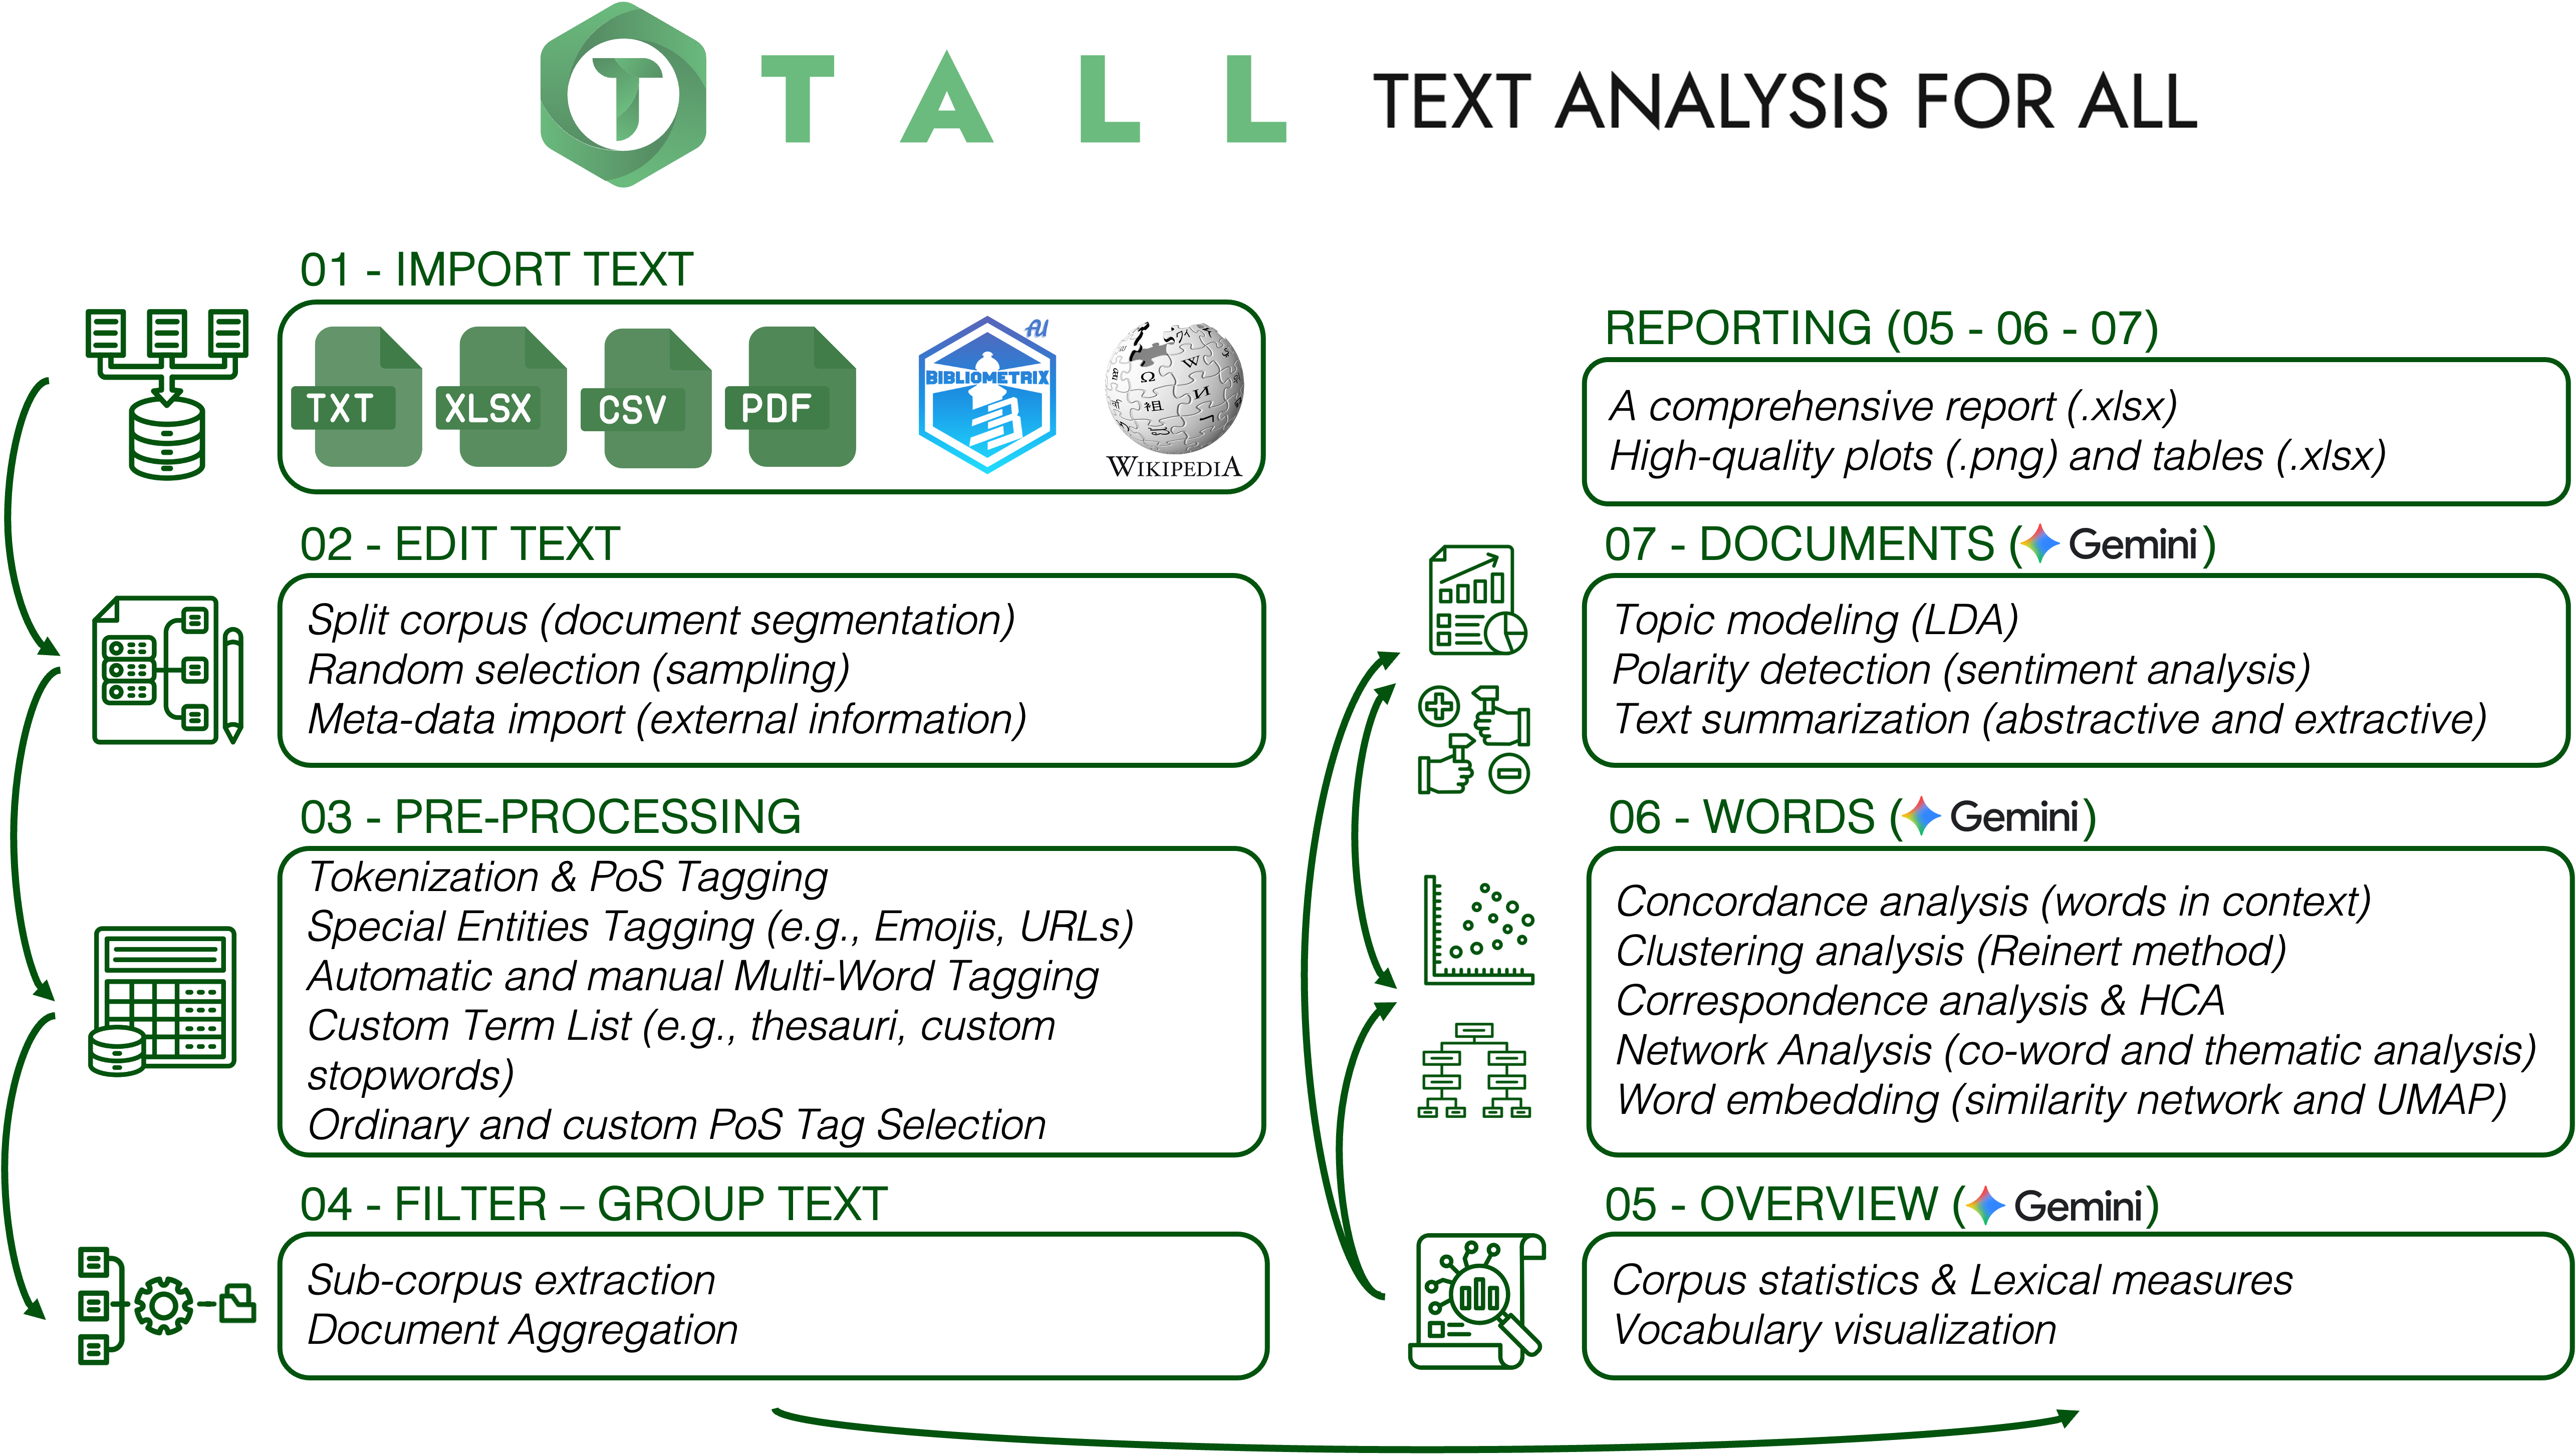
\includegraphics[width=0.95\textwidth]{workflow.png}}
\caption{TALL workflow and main components.}
\label{fig:0}
\end{figure}

\subsection{Software functionalities}
TALL integrates an end-to-end text mining workflow into a unified and interactive graphical environment. The application is designed to guide the user through the entire process of textual data analysis, from data import to result interpretation, within an intuitive, tab-oriented \textsf{R}-Shiny interface. The overall structure is organized into three main layers: \textit{Data Import and Management}, \textit{Text Pre-processing}, and \textit{Analysis}. These layers correspond to the logical stages of a typical computational text analysis pipeline, schematically depicted in Fig.~\ref{fig:0}. This modular structure enables users to explore each stage while maintaining the continuity of the data flow.

\paragraph{Data import and management}
The first layer handles the acquisition, inspection, and preparation of the textual corpus. TALL accepts a broad range of input formats $-$ including plain text (\textsf{.txt}), comma-separated files (\textsf{.csv}), spreadsheets (\textsf{.xlsx}), and Portable Document Format (\textsf{.pdf}) $-$ and automatically detects character encoding to prevent loss of diacritical or non-ASCII characters. Metadata can be uploaded in parallel with the textual content, allowing users to associate attributes such as author, publication source, thematic label, or date with each text unit. The metadata can later serve as filters or grouping factors in downstream analyses. Moreover, TALL is integrated with the \textsf{bibliometrix} package to analyze scientific publication collections, accepting as input \textsf{biblioshiny} files as well. Within the same interface, a \textit{Data Editor} panel provides a reactive table view that supports row filtering, text search, and random or stratified sampling. The segmentation utility enables the partitioning of large \textit{corpora} into smaller textual units, such as paragraphs, records, or user-defined delimiters. These functionalities enable users to verify data integrity and structure prior to text preprocessing. The interface also allows dynamic saving of edited \textit{corpora}, ensuring that early-stage manipulations are retained for subsequent sessions.

\begin{figure}[!ht]
\centering
\fbox{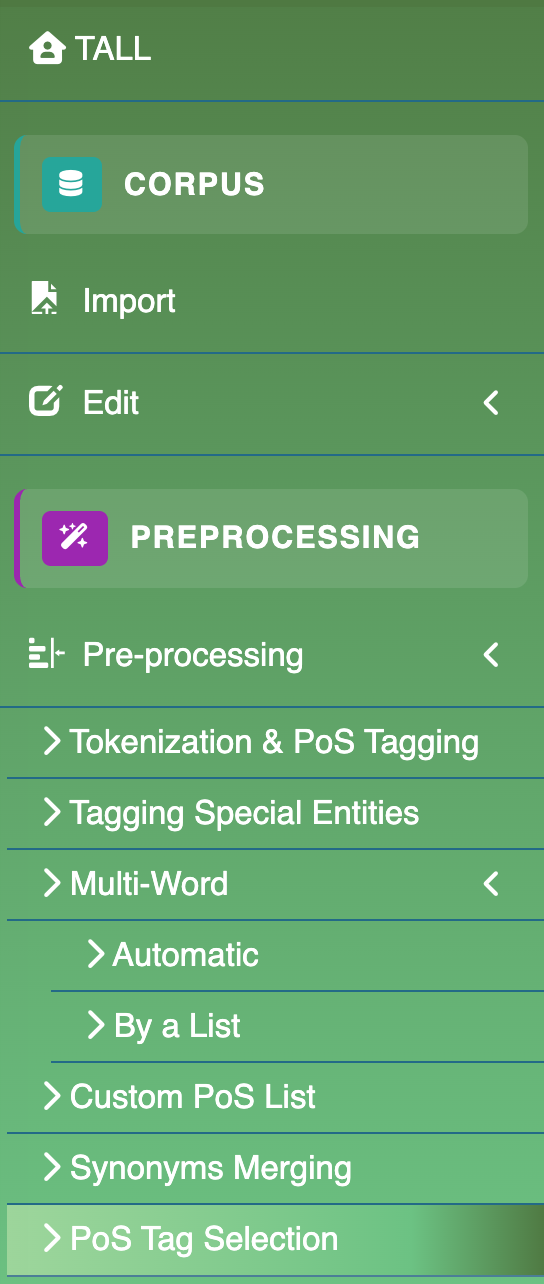
\includegraphics[width=0.35\textwidth]{menu.png}}
\caption{Navigation sidebar of the TALL app: Import and Pre-processing modules.}
\label{fig:1}
\end{figure}

\paragraph{Text pre-processing}
The pre-processing layer standardizes and transforms raw text into structured representations suitable for quantitative analysis (Fig.~\ref{fig:1}. Core operations include \textit{tokenization}, \textit{PoS tagging}, and \textit{lemmatization}. These tasks are implemented through the \textsf{udpipe} package \cite{wij25}, accessing the set of 87 \textit{ad hoc} pre-trained language models. The selected model is downloaded and cached locally to enhance performance and facilitate offline processing. For domain-specific adaptation, users may upload custom dictionaries, thesauri, or stopword lists, which can refine lemmatization and lexical normalization. An additional utility allows both the automatic and manual creation of multi-word expressions (\textit{n-grams}). TALL integrates four algorithms for identifying salient collocations and candidate keyphrases based on co-occurrence statistics, including the \textit{Rapid Automatic Keyword Extraction} (RAKE) algorithm \cite{ros10}.

\paragraph{Analysis and visualization modules}
The analytical layer provides a comprehensive suite of statistical and graphical modules, each implemented as an independent sub-menu that can be executed separately or in sequence. Analyses can be performed on tokens or lemmas. The TALL AI assistant generates natural-language explanations of outputs, contextual comments, and narrative summaries of results. The generated commentary appears in collapsible panels alongside numerical or graphical outputs, providing interpretive context that enhances accessibility for non-specialist users. The \textit{Overview} tab presents descriptive statistics on the analyzed collection, including frequency distributions, lexical richness, and term-weighting measures. The TF-IDF (\textit{term frequency–inverse document frequency}) sub-tab refines term relevance \cite{sal88}, highlighting discriminating words across document sets. Word frequency plots and word clouds, generated using the \textsf{plotly} library \cite{sie20}, support zooming and tooltip interactions. The analytical layer distinguishes between word- and document-level analyses, guiding users toward the most suitable approach. Within the \textit{Words} menu, several methods support the exploration of a \textit{corpus} semantic space. \textit{Words in Context} enables the analysis of concordances and co-text environments, facilitating qualitative interpretation of usage patterns \cite{wul20}; \textit{Reinert Clustering} implements the hierarchical descending clustering proposed by M.~Reinert \cite{rei83}, generating lexically homogeneous clusters from co-occurrence patterns; \textit{Correspondence Analysis} $-$ executed via the \textsf{ca} package \cite{nen07} $-$ reveals latent semantic dimensions; the \textit{Network} module performs co-occurrence analysis using the \textsf{igraph} \cite{csa06} and \textsf{visNetwork} \cite{alm25} packages; \textit{Word Embeddings} computes high-dimensional vector representations through the \textsf{word2vec} package \cite{wij23}, allowing exploration of semantic relationships among terms. The \textit{Document} menu includes three main modules: \textit{Topic Modeling}, based on \textit{Latent Dirichlet Allocation} (LDA) \cite{ble03} and implemented with the \textsf{topicmodels} package \cite{gru11}, estimates thematic structures across the \textit{corpus}; \textit{Polarity Detection} evaluates emotional valence using sentiment lexicons such as Loughran–McDonald \cite{lou16} and NRC \cite{moh13}, producing visual dashboards of sentiment distributions across documents and topics; and \textit{Summarization} extracts key sentences via the \textsf{textrank} package \cite{wij20}, facilitating concise content overviews. Abstractive summarization can also be performed.

\begin{figure}[!ht]
\centering
\fbox{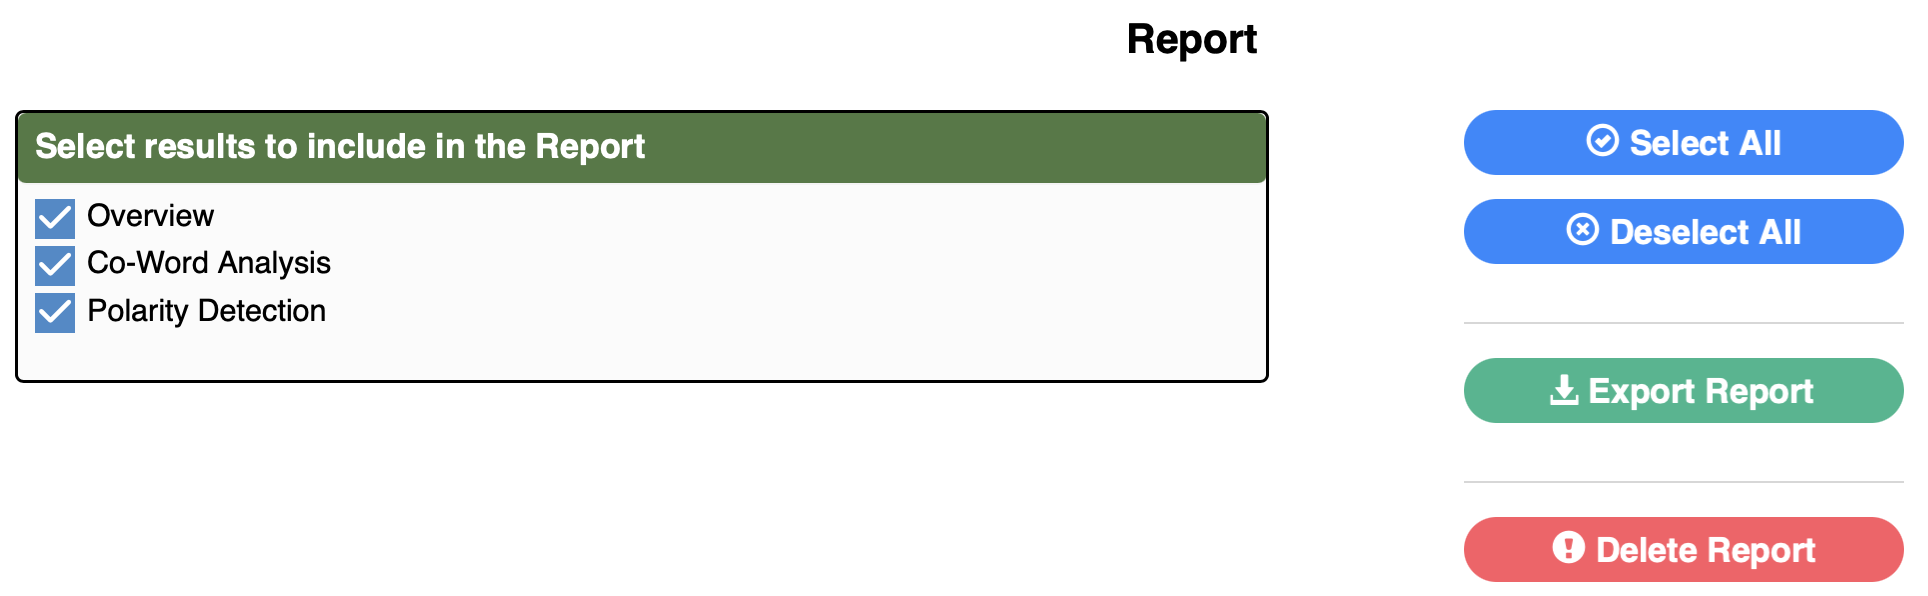
\includegraphics[width=0.95\textwidth]{report.png}}
\caption{Interface for report customization showing selected outcomes and options.}
\label{fig:rep}
\end{figure}

The numerical and graphical results are exportable in multiple formats. All the tables and statistics can be downloaded as \textsf{.csv} or \textsf{.xlsx} files, whereas visualizations can be downloaded as \textsf{.png} outputs. Moreover, it is possible to assemble the various outcomes of the analytical layer into a comprehensive report (Fig.~\ref{fig:rep}) that can be exported as a single \textsf{.xlsx} file.

\section{Illustrative examples}
To demonstrate the capabilities of TALL, two examples based on publicly available datasets included in the application are presented. These examples illustrate how users can perform complete analytical workflows $-$ from data import to interpretation $-$ without writing any code.

\subsection{Example 1: Thematic analysis on BBC news}
The first example uses a set of 386 short news from the \textit{BBC News corpus}, a collection of English-language stories retrieved from the BBC website \cite{gre05}. After loading the \textit{corpus}, standard pre-processing steps are applied through the \textit{Pre-processing} menu, including tokenization and lemmatization via the EN \textsf{GUM} model. Adjectives, nouns, proper nouns, and verbs are retained by default. In the \textit{Overview} menu (Fig.~\ref{fig:2}, \textit{corpus} statistics and lexical diversity measures provide an initial characterization of the collection. 

\begin{figure}[!ht]
\centering
\fbox{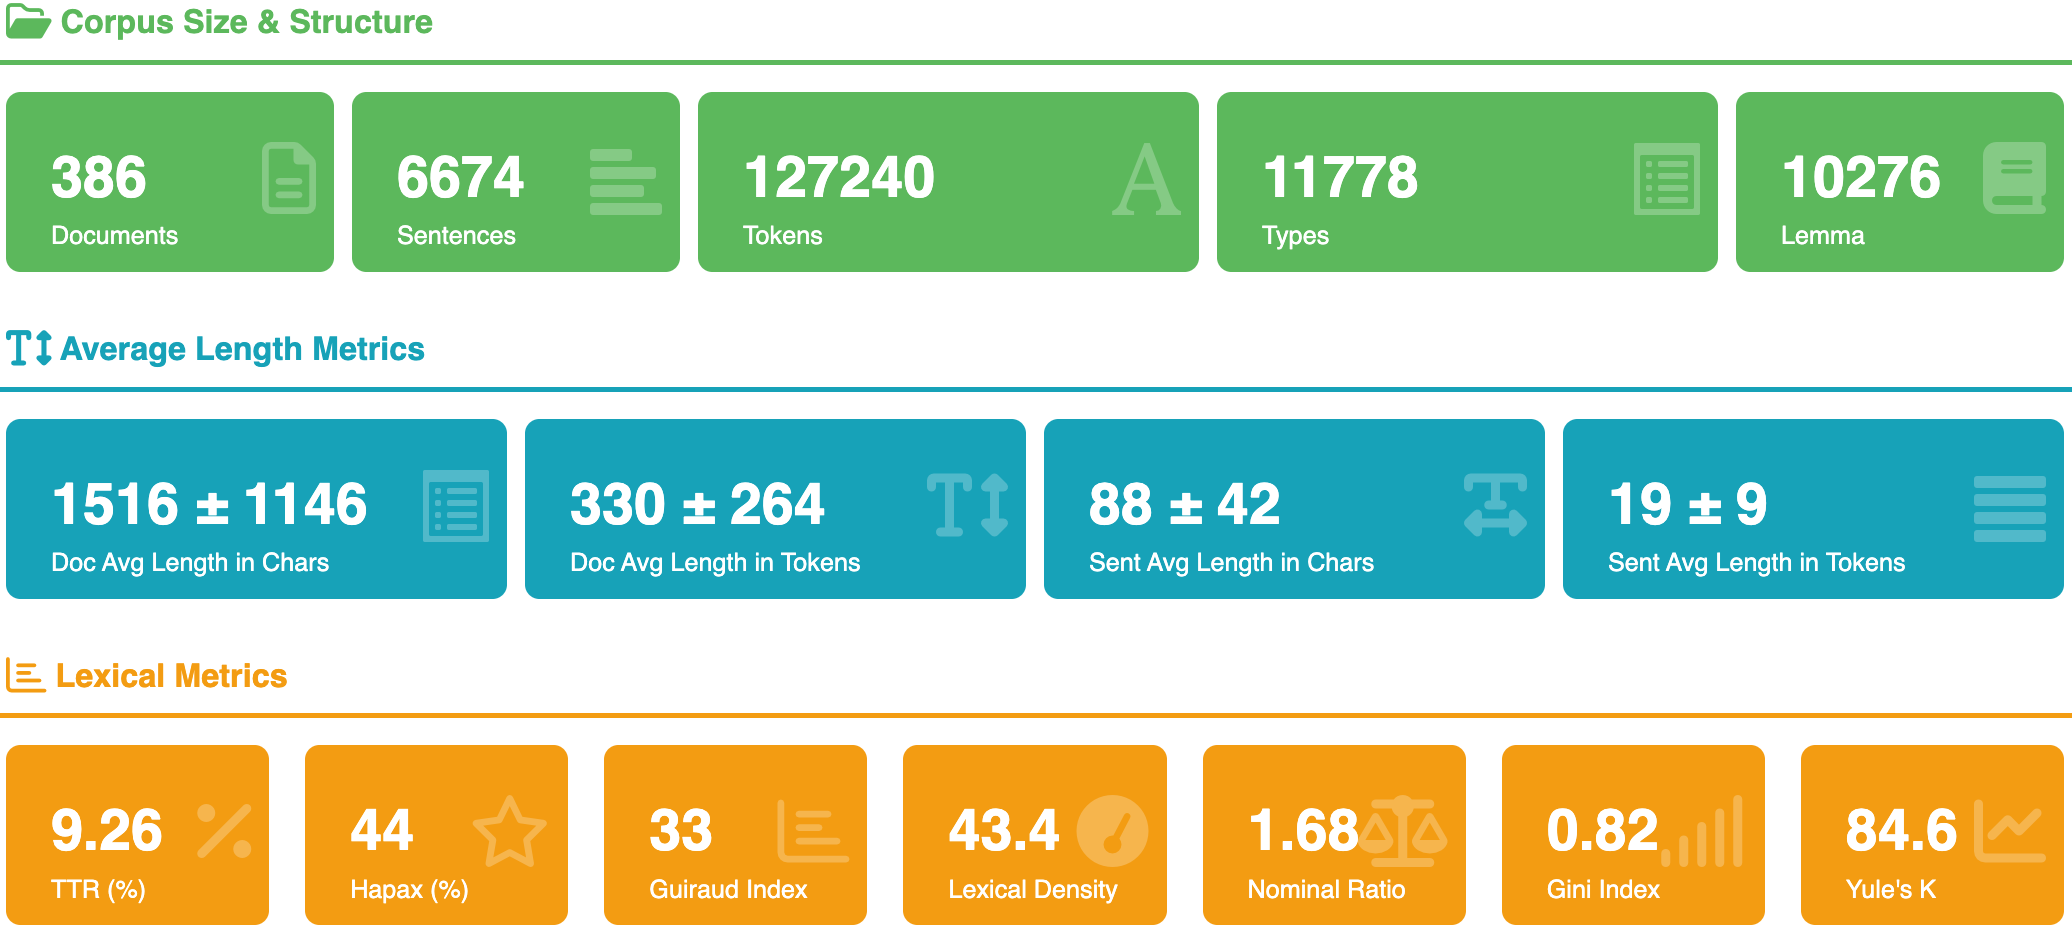
\includegraphics[width=0.95\textwidth]{overview.png}}
\caption{Descriptive statistics of the BBC News entertainment sub-\textit{corpus}.}
\label{fig:2}
\end{figure}

The \textit{Network} module highlights the main co-occurrence relationships among terms. After segmenting each document into sentences, a community detection algorithm is applied to the adjacency matrix of the top 100 lemmas' co-occurrences, identifying five dense sub-graphs (Fig.~\ref{fig:3}).

\begin{figure}[!ht]
\centering
\fbox{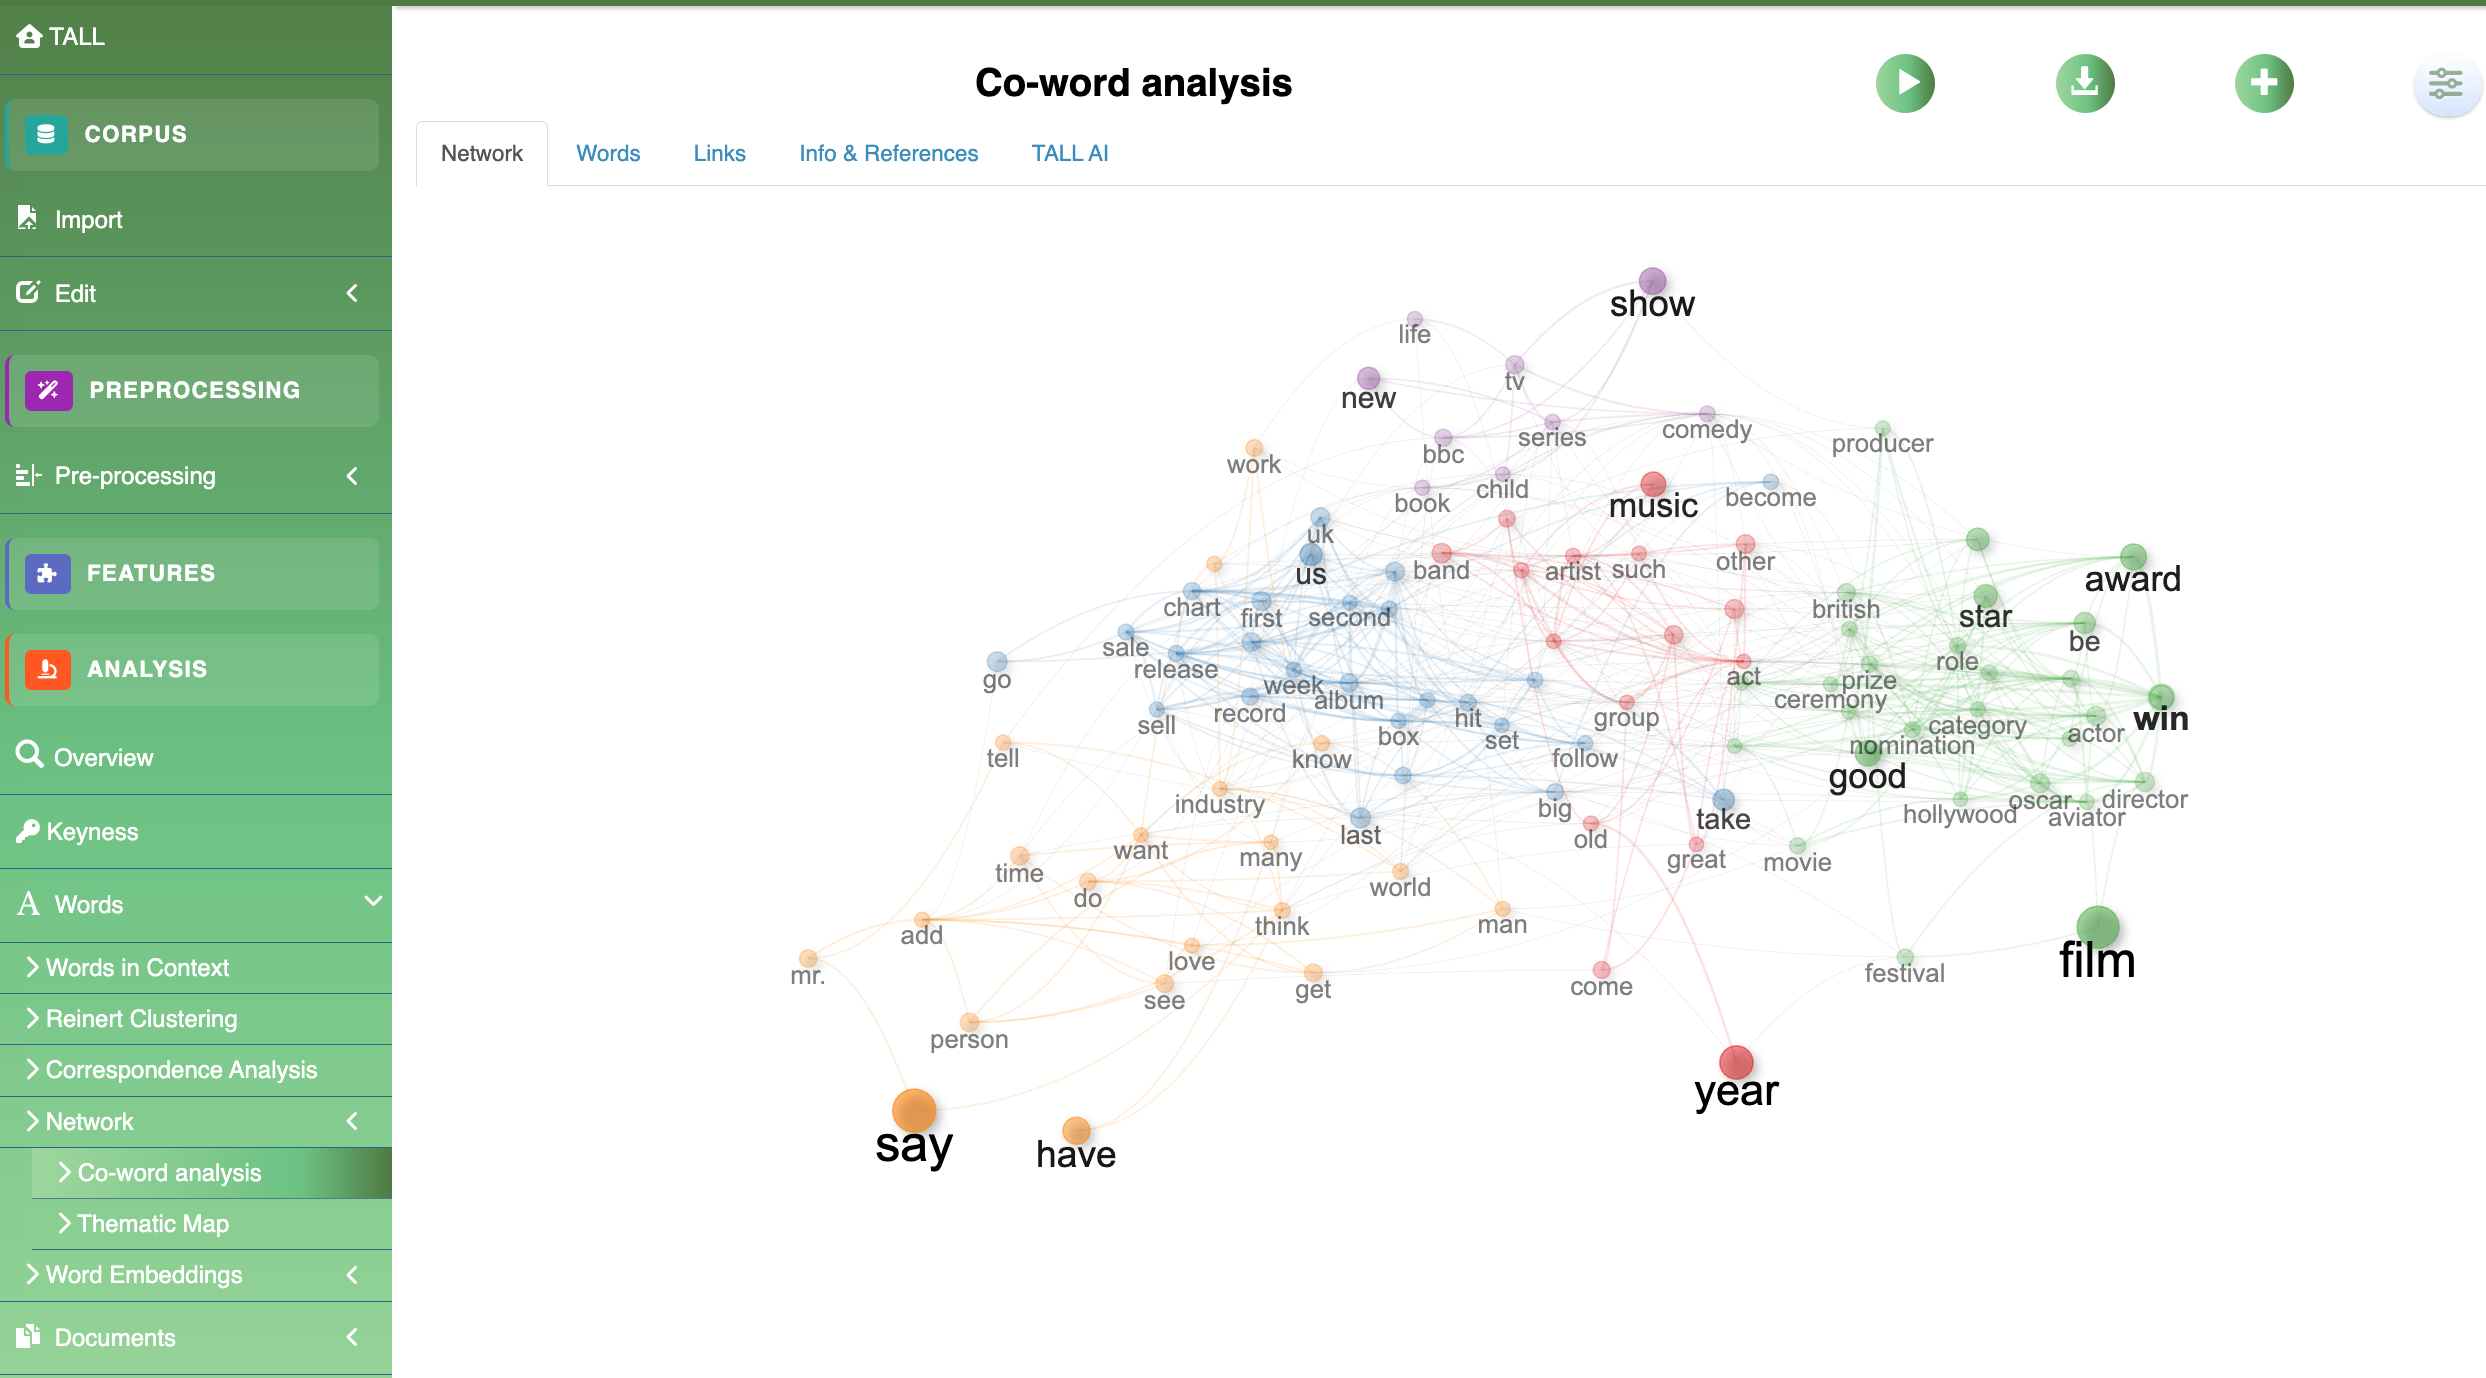
\includegraphics[width=0.95\textwidth]{network_mod.png}}
\caption{Community detection on the BBC News entertainment sub-\textit{corpus}.}
\label{fig:3}
\end{figure}

With the help of TALL AI, we interpret the five sub-graphs as topical clusters: \textit{Awards/Movies} (green cluster), \textit{Music and Performance} (red cluster), \textit{Music Industry and Sales} (blue cluster), \textit{Media and Entertainment Coverage} (purple cluster), \textit{General News} (orange cluster).
 We can also gain some insights via TALL AI (e.g., \textit{the entertainment news focuses heavily on film awards and the movie industry}; \textit{music-related news is a significant portion of the content}).

\subsection{Example 2: Sentiment detection on US Airline Tweets}
The second example employs the \textit{US Airline Tweets corpus}, which contains 14,640 tweets directed at six major American airlines in February 2015 \cite{fig15}. 

After loading the \textit{corpus}, standard pre-processing steps are applied through the \textit{Pre-processing} sub-menu, including tokenization and lemmatization via the EN \textsf{EWT} model. Hashtags detected in the \textit{Tagging Special Entities} sub-menu are retained, along with adjectives, nouns, and proper nouns. Within the \textit{Polarity Detection} module, sentiment analysis is performed using the NRC Emotion Lexicon. The resulting dashboards display the distribution of sentiment across airlines, showing that negative tweets are predominantly associated with service disruptions and delays (Fig.~\ref{fig:4}). 

\begin{figure}[!ht]
\centering
\fbox{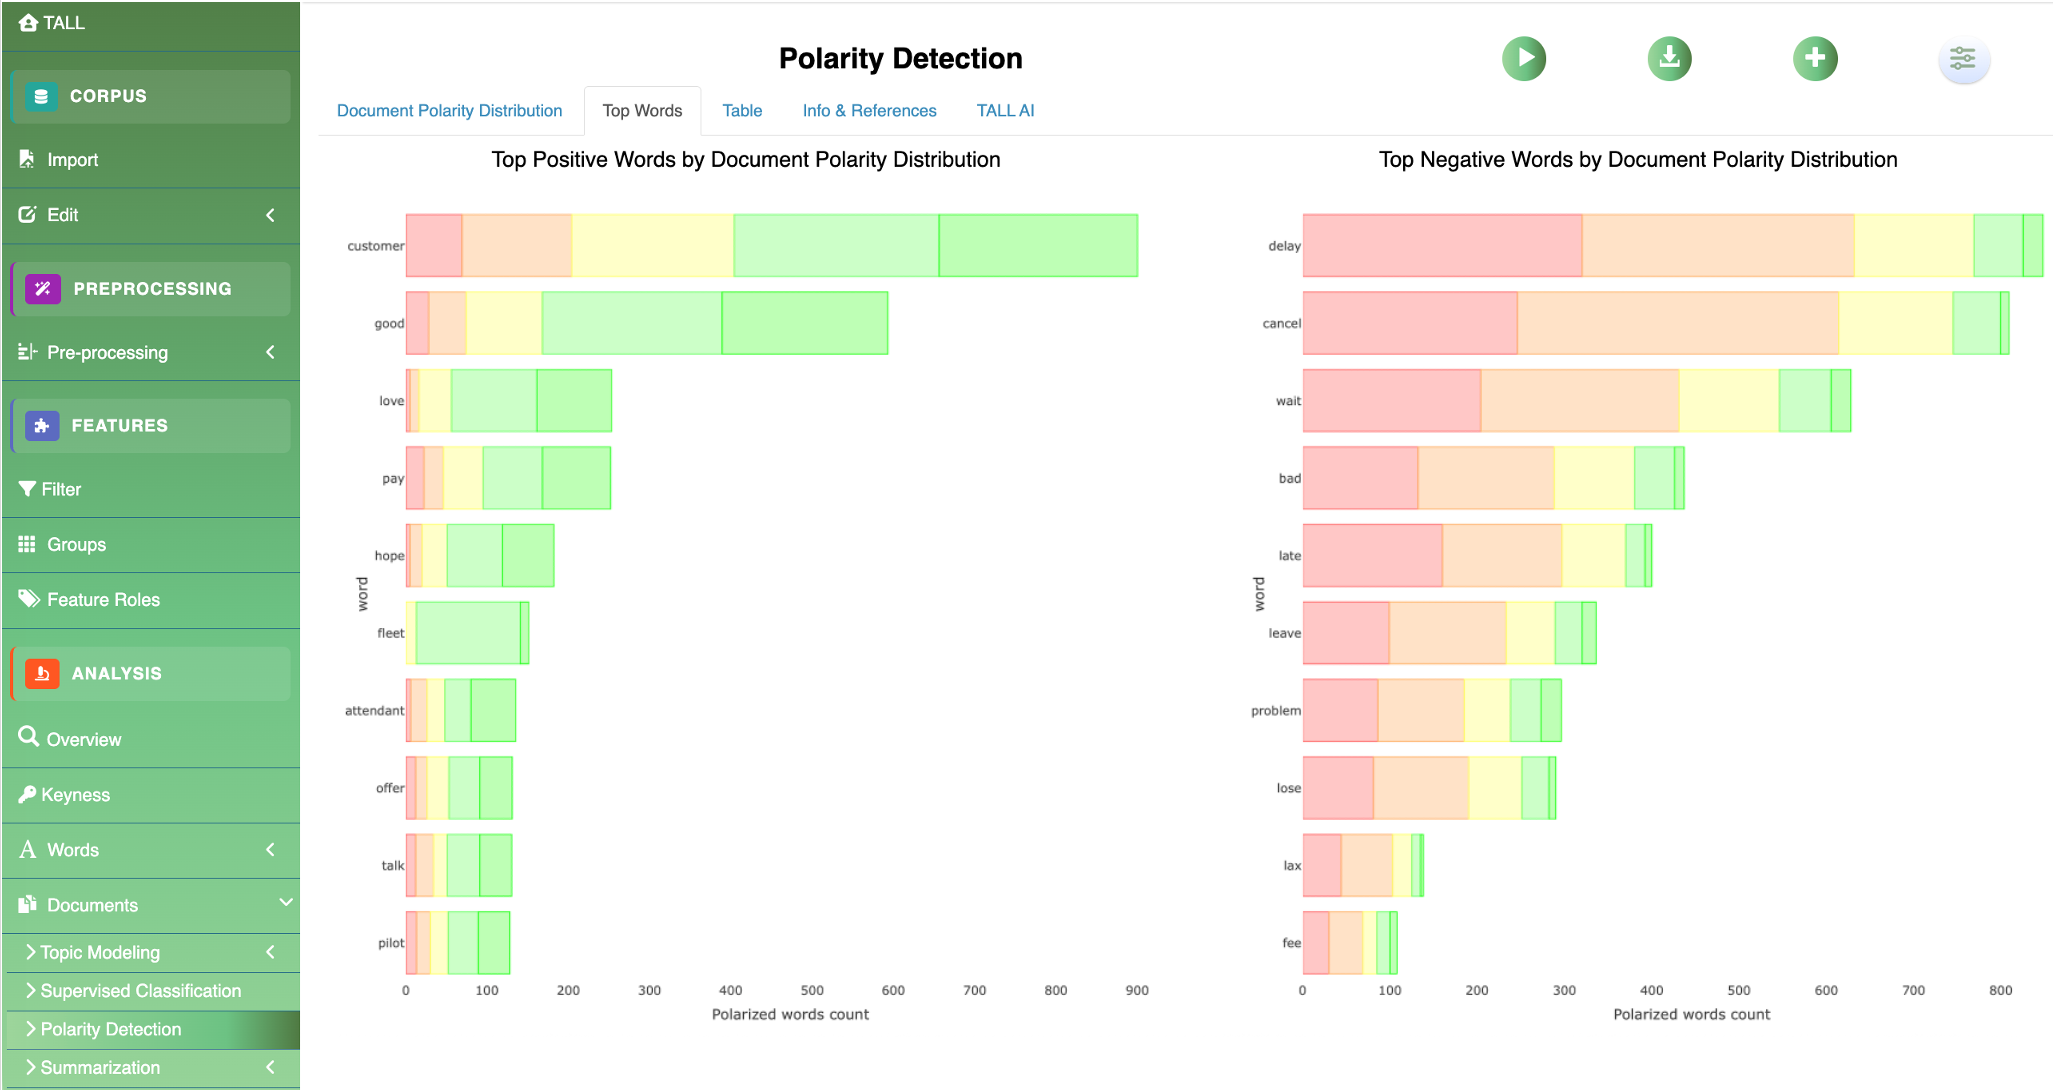
\includegraphics[width=0.95\textwidth]{sentiment_mod.png}}
\caption{Top word distributions by document polarity in the US Airline Tweets \textit{corpus}.}
\label{fig:4}
\end{figure}

In TALL AI comments, it is possible to find \textit{Key Takeaways \& Implications} derived from the outcomes of the analysis: e.g, \textit{the dominance of 'delay' and 'cancel' in negative tweets suggests airlines should focus on improving their processes for handling flight disruptions (...)}; \textit{both positive and negative tweets highlight the importance of customer service (...)}. By selecting sub-sets of positive or negative documents, users can further examine common lexical patterns using, for example, \textit{Words in Context} or \textit{Topic Modeling} modules.

A step-by-step workflow example on the US Airline Tweets dataset is available in the supplementary material.

\section{Impact and conclusions}
TALL advances reproducible and transparent analysis of textual data by integrating NLP and text mining methods into a unified, open-source environment. The application operationalizes the FAIR data principles through explicit documentation of each analytical step, persistent repositories, and interoperable export formats. Each module is accompanied by metadata that describes the algorithms and parameters, ensuring that both human and machine agents can reproduce the analytical process. The combination of classical methods $-$ such as correspondence analysis and topic modeling $-$ with recent advances in word embeddings and network analytics enables multimodal language exploration. The embedded TALL AI assistant introduces AI-assisted interpretation of results, generating textual explanations and fostering interaction between statistical evidence and linguistic reasoning. This hybrid human–machine approach stimulates new research directions in semantic modeling, interpretability, and evaluation of generative language models within controlled analytical workflows.

TALL enhances the investigation of research questions in fields in which unstructured text is a primary empirical source. In social and political sciences, it supports large-scale thematic and sentiment analyses of institutional reports or online debates. In science mapping, the integration with the \textsf{bibliometrix} package allows the combination of semantic and citation-based analyses. In digital humanities, the multilingual architecture based on our \textit{ad hoc} pre-trained models enables cross-linguistic \textit{corpus} studies and cultural analyses. By lowering technical barriers, TALL extends the reach of NLP to communities that have traditionally lacked computational resources, promoting methodological inclusivity and reproducibility in qualitative inquiry. Evidence of its early impact is already visible: its role as an application for non-programmers has been emphasized in \cite{san24,tay25}, and it has been applied in empirical studies using textual data \cite{val25}. TALL is currently employed in postgraduate and doctoral programs at several Italian universities, supporting the teaching of data-driven methods in social sciences and computational linguistics. The package has been officially published on the \textit{Comprehensive R Archive Network} (CRAN) (\url{https://cran.r-project.org/package=tall}), ensuring long-term accessibility and compliance with \textsf{R} standards. According to CRANlogs, TALL has exceeded 4,000 downloads since its release (February, 2025), denoting growing interest within the research community. This diffusion underscores the app's utility and reliability for text mining and NLP tasks. CRAN publication also guarantees version control and continuous integration within the \textsf{R} ecosystem, enhancing interoperability with other open-source resources. By coupling algorithmic transparency with accessibility, TALL consolidates the methodological foundations of text analytics as a reproducible scientific practice, positioning itself as an extensible infrastructure for interdisciplinary NLP research. 

TALL is designed as a desktop application for standalone personal computers, with computational constraints inherent in the user's hardware specifications (processor speed, available RAM). While we have implemented multiple optimization strategies to enhance computational efficiency (see Section 2.1), very large \textit{corpora} may require server deployment for practical processing times. A key advantage of TALL's web-based architecture is scalability: the same application can be seamlessly deployed on institutional Shiny Server infrastructure, enabling analysis of large-scale \textit{corpora} without modifying the codebase or user interface. This architectural flexibility allows TALL to serve both individual researchers working with modest datasets on personal laptops and research groups requiring centralized, high-performance text analysis infrastructure. TALL's AI integration requires privacy evaluation for confidential research. Despite only aggregated statistics are transmitted, these may reveal sensitive patterns in small \textit{corpora}. For regulated data (e.g., EU-GDPR, US-HIPAA), it is recommended to: (1) disable TALL AI; (2) isolated server deployment; or (3) anonymize data. In any case, it would be necessary to consult institutional review boards for human subjects research. Future versions may support local language models to enhance privacy management.

The development team maintains TALL through regular updates on GitHub and CRAN, ensuring compatibility with future \textsf{R} releases and the incorporation of emerging NLP and visualization libraries. Future versions will enhance interoperability through API endpoints for external datasets and connectors to cloud-based repositories (e.g., Kaggle), thereby improving scalability and facilitating collaborative research.

%%%%%%%%%%%%%%%%%%%%%%%%%%%%%%%%%%%%%%%%%%%%%%%%%%%%%%%%%%%%%%

\footnotesize{
\section*{CRediT authorship contribution statement}
\textbf{MA}, \textbf{MS}, \textbf{LD}: Conceptualization, Methodology, Software, Data curation, Resources, Validation, Writing -- review \& editing. \textbf{CC}: Conceptualization, Validation, Writing -- review \& editing. \textbf{MM}: Conceptualization, Methodology, Validation, Writing -- original draft, Writing -- review \& editing.

\section*{Declaration of competing interest}
The authors declare that they have no known competing financial interests or personal relationships that could have appeared to influence the work reported in this paper.

\section*{Data availability}
The code and data used in this paper can be retrieved from the repositories in \url{https://github.com/massimoaria}

\section*{Supplementary materials}
Supplementary material associated with this article can be found in the online version at XXX.

\section*{Acknowledgement}
This research has been financed by the following research projects: PRIN-2022  (Project Code:2022825Y5E; CUP:E53D2300611006) -- \textit{SCIK-HEALTH}; PRIN-2022 PNRR  (Project Code:P2022RF38Y; CUP:E53D23016650001) -- \textit{The value of scientific production for patient care in Academic Health Science Centres}.
}

%%%%%%%%%%%%%%%%%%%%%%%%%%%%%%%%%%%%%%%%%%%%%%%%%%%%%%%%%%%%%%

\begin{thebibliography}{00}

\bibitem{alm25}
Almende BV and Contributors, Thieurmel B. visNetwork: Network Visualization using 'vis.js' Library. 2025, \url{https://doi.org/10.32614/CRAN.package.visNetwork}, R package version 2.1.4.

\bibitem{ant24}
Anthony, L. (2024). AntConc. Version 4.3.1 [software]. 2024 Jul 29. \url{https://www.laurenceanthony.net/software/AntConc}.

\bibitem{ari17} Aria M, Cuccurullo C. bibliometrix: An R-tool for comprehensive science mapping analysis. J Informetr 2017;11(4):959-975 \url{https://doi:10.1016/j.joi.2017.08.007}.

\bibitem{ari22} Aria M, Cuccurullo C, D'Aniello L, Misuraca M, Spano M. Thematic Analysis as a New Culturomic Tool: The Social Media Coverage on COVID-19 Pandemic in Italy. Sustainability 2022;14(6):3643. \url{https://doi.org/10.3390/su14063643}.

\bibitem{ari25} Aria M. Pre-trained models for TALL. 2025, \url{https://github.com/massimoaria/tall.language.models} 

\bibitem{ben21} Bengtsson H. A Unifying Framework for Parallel and Distributed Processing in R using Futures. R J 2021;13(2):208–227. \url{https://doi.org/10.32614/RJ-2021-048}.

\bibitem{ble03} Blei DM, Ng AY, Jordan MI. Latent Dirichlet Allocation. J Mach Learn Res 2003;3(Jan):993–1022. \url{https://www.jmlr.org/papers/volume3/blei03a/blei03a.pdf}.

\bibitem{che05} Chen H, Fuller SS, Friedman C, Hersh W. Knowledge Management, Data Mining, and Text Mining in Medical Informatics. In: Chen H, Fuller SS, Friedman C, Hersh W, editors. Medical Informatics. Integrated Series in Information Systems, Boston, MA: Springer; 2005, p. 3-33. \url{https://doi.org/10.1007/0-387-25739-X_1}.

\bibitem{che25} Cheng J. promises: Abstractions for Promise-Based Asynchronous Programming. 2025, \url{https://doi.org/10.32614/CRAN.package.promises}, R package version 1.3.3.

\bibitem{csa06} Cs{\'a}rdi G, Nepusz T. The igraph software package for complex network research. InterJournal, Complex Syst 2006;1695. \url{https://igraph.org}.

\bibitem{dem21} de Marneffe MC, Manning C, Nivre J, Zeman D. Universal Dependencies. Comput Linguist 2021;47(2):255-308. \url{https://doi.org/10.1162/coli_a_00402}.

\bibitem{dim15} DiMaggio P. Adapting computational text analysis to social science (and vice versa). Big Data Soc 2015; 2(2):2053951715602908. \url{https://doi.org/10.1177/2053951715602908}.

\bibitem{feu25} Feuerriegel S, Maarouf A, B{\"a}r D, Geissler D, Schweisthal J, Pr{\"o}llochs N, et al. Using natural language processing to analyse text data in behavioural science. Nat Rev Psychol 2025;4:96–111. \url{https://doi.org/10.1038/s44159-024-00392-z}.

\bibitem{fig15} Figure Eight. Twitter US Airline Sentiment [dataset]. Kaggle Data. 2015. \url{https://www.kaggle.com/datasets/crowdflower/twitter-airline-sentiment}

\bibitem{for16} Fortunato S, Hric D. Community detection in networks: A user guide. Phys Rep 2016;659:1–44. \url{https://doi.org/10.1016/j.physrep.2016.09.002}.

\bibitem{gre05} Greene D, Cunningham P. BBC News [dataset]. ML Resources UCD. 2005. \url{http://mlg.ucd.ie/datasets/bbc.html}

\bibitem{gru11} Gr{\"u}n B, Hornik K. topicmodels: An R Package for Fitting Topic Models. J Stat Softw 2011;40(13):1–30. \url{https://doi.org/10.18637/jss.v040.i13}.

\bibitem{hig17} Higuchi K. New Quantitative Text Analytical Method and KH Coder Software. Jpn Sociol Rev 2017;68(3):334-350. \url{https://doi.org/10.4057/jsr.68.334}.

\bibitem{ign16} Ignatow G. Theoretical Foundations for Digital Text Analysis. J Theory Soc Behav 2016;46(1):104-120. \url{https://doi.org/10.1111/jtsb.12086}.

\bibitem{lou16} Loughran T, McDonald B. Textual analysis in accounting and finance: A survey. J Account Res 2016;54(4):1187–1230. \url{https://doi.org/10.1111/1475-679X.12123}.

\bibitem{mis20} Misuraca M, Spano M. Unsupervised Analytic Strategies to Explore Large Document Collections. In: Iezzi DF, Mayaffre D, Misuraca M, editors. Text Analytics, Advances and Challenges, Cham: Springer; 2020, p. 17–28. \url{https://doi.org/10.1007/978-3-030-52680-1_2}.

\bibitem{moh13} Mohammad SM, Turney DP. Crowdsourcing a word-emotion association lexicon. Comput Intell 2013;29(3):436-465. \url{https://doi.org/10.1111/j.1467-8640.2012.00460.x}.

\bibitem{nen07} Nenadić O, Greenacre M. Correspondence analysis in R, with two- and three-dimensional graphics: The ca package. J Stat Softw 2007;20(3):1–13. \url{https://doi.org/10.18637/jss.v020.i03}.

\bibitem{rat14} Ratinaud P. IRAMUTEQ: Interface de R pour les analyses multidimensionnelles de textes et de questionnaires. Version 0.8 alpha 7 [software]. 2024 Nov 2. \url{http://www.iramuteq.org}.

\bibitem{rei83} Reinert M. Une m{\'e}thode de classification descendante hi{\'e}rarchique: application {\`a} l'analyse lexicale par contexte. Cah Anal Donn 1983;8(2):187-198 (1983). \url{https://www.numdam.org/item/CAD_1983__8_2_187_0}.

\bibitem{ros10} Rose S, Engel D, Cramer N, Cowley W. Automatic keyword extraction from individual documents. In: Berry MW, Kogan J, editors. Text Mining: Applications and Theory. Chichester: Wiley; 2010. p. 1–20. \url{https://doi.org/10.1002/9780470689646.ch1}.

\bibitem{sal88} Salton G, Buckley C. Term-weighting approaches in automatic text retrieval. \textit{Inf Process Manage} 1988;24(5):513–523. \url{https://doi.org/10.1016/0306-4573(88)90021-0}.

\bibitem{san24} Santosa FA, Lamba M, George C, Downie JS. Coconut Libtool: Bridging Textual Analysis Gaps for Non-Programmers. Proc Assoc Inf Sci Technol 2024;61(1):639-644. \url{https://doi.org/10.1002/pra2.1072}.

\bibitem{sie20} Sievert C. Interactive Web-Based Data Visualization with R, plotly, and shiny. Boca Raton, FL: Chapman \& Hall/CRC; 2020. \url{https://doi.org/10.1201/9780429447273}.

\bibitem{tab11} Taboada M, Brooke J, Tofiloski M, Voll K, Stede M. Lexicon based methods for sentiment analysis. Comput Linguist 2011;37(2):267–307. \url{https://aclanthology.org/J11-2001/}.

\bibitem{tay25} Tay A. TALL - Text Analysis for ALL - New R Shiny, \url{https://library.smu.edu.sg/topics-insights/tall-text-analysis-all-new-r-shiny}; 2025 [accessed 17 October 2025].

\bibitem{val25} Valentino C, Aria M, Angelelli M, Ciavolino E. Patient satisfaction and healthcare quality perception: an explorative textual analysis. In: Boccuzzo G, Bovo E, Manisera M, Salmaso L. Innovation \& Society -- Statistics and Data Science for Evaluation and Quality. Padua: Cleup; 2025. p. 552-557.

\bibitem{wij20} Wijffels J. textrank: Summarize Text by Ranking Sentences and Finding Keywords. 2020. \url{https://CRAN.R-project.org/package=textrank}, R package version
0.3.1.

\bibitem{wij23} Wijffels J, Watanabe K. word2vec: Distributed Representations of Words. 2023. \url{https://CRAN.R-project.org/package=word2vec}, R package version 0.4.0.

\bibitem{wij25} Wijffels J. udpipe: Tokenization, Parts of Speech Tagging, Lemmatization and Dependency Parsing with the 'UDPipe' 'NLP' Toolkit. 2025. \url{https://doi.org/10.32614/CRAN.package.udpipe}, R package version 0.8.12.

\bibitem{wil16} Wilkinson MD, Dumontier M, Aalbersberg IJ, Appleton G, Axton M, Baak A, et al. The FAIR Guiding Principles for scientific data management and stewardship. Sci Data 2016;3:160018. \url{https://doi.org/10.1038/sdata.2016.18}.

\bibitem{wul20} Wulff S, Baker P. Analyzing Concordances. In: Paquot M, Gries ST, editors. A Practical Handbook of Corpus Linguistics, Cham: Springer; 2020, p. 161–179. \url{https://doi.org/10.1007/978-3-030-46216-1_8}.

\end{thebibliography}

\end{document}
\endinput
%%
%% End of file `SoftwareX_article_template.tex'.

%%% Local Variables:
%%% mode: latex
%%% TeX-master: t
%%% End:
